Nesse capítulo, serão apresentados os resultados obtidos utilizando o método multiescala para solução dos sistemas lineares decorrentes do operador apresentado em \ref{ch:modelagem}. Os resultados são apresentados na seguinte ordem: resultados em casos que a solução analítica é conhecida para testar o bom funcionamento do método, comparações do método multiescala como pré-condicionador e resultados do método multiescala como solver linear.


\section{Soluções Analíticas}

Para atestar o bom resultado do método, é importante comparar com soluções que são conhecidas analiticamente. Os testes apresentados são incrementais de forma a testar que todas as opções estão funcionando corretamente.

Primeiro, são apresentados casos onde as condições de contorno são de Dirichlet Homogêneas. Esse teste é aplicado no domínio $ \Omega = [0, 2] \times [0, 2]$ com solução apresentada em \ref{eq:solucaoDirichletHomogeneo};

\begin{equation}\label{eq:solucaoDirichletHomogeneo}
u = 
\begin{bmatrix}
u_x
\\ 
u_y
\end{bmatrix}
=
\begin{bmatrix}
y(-y+2)sen(\pi x))
\\ 
x(-x+2)sen(\pi x))
\end{bmatrix}
\end{equation}É importante notar que os valores da solução na fronteira do domínio são zero. Pode-se calcular o lado direito referente dessa solução aplicando o operador do problema. Fazendo isso, o lado direito encontrado é o mostrado em \ref{eq:ldDiricheletHomogeneo}.

\begin{equation}\label{eq:ldDiricheletHomogeneo}
f(x, y) = 
\left[\begin{matrix}
\begin{split}
\frac{\pi E v x}{v^{2} - 1} \cos{\left (\pi y \right )} - \frac{\pi E v}{v^{2} - 1} \left(- x + 2\right) \cos{\left (\pi y \right )} + \frac{\pi^{2} E y}{v^{2} - 1} \left(- y + 2\right) \sin{\left (\pi x \right )} 
\\
+
\frac{E}{2 v + 2} \left(- \pi x \cos{\left (\pi y \right )} + \pi \left(- x + 2\right) \cos{\left (\pi y \right )} - 2 \sin{\left (\pi x \right )}\right)
 \end{split}
\\

\frac{\pi E v y}{v^{2} - 1} \cos{\left (\pi x \right )} - \frac{\pi E v}{v^{2} - 1} \left(- y + 2\right) \cos{\left (\pi x \right )} 
\\
+ \frac{\pi^{2} E x}{v^{2} - 1} \left(- x + 2\right) \sin{\left (\pi y \right )} + \frac{E}{2 v + 2} \left(- \pi y \cos{\left (\pi x \right )} + \pi \left(- y + 2\right) \cos{\left (\pi x \right )} - 2 \sin{\left (\pi y \right )}\right)\end{matrix}\right]
\end{equation}


Assim, o problema \ref{eq:problemaDirichlet}.

\begin{equation} \label{eq:problemaDirichlet}
    x = 1
\end{equation}

A figura \ref{fig:DirichletHomogeneo} apresenta a comparação entre a solução de um grid fino contra a solução do grid grosso.  

\begin{figure}[!htbp]
\label{fig:DirichletHomogeneo}
\centering
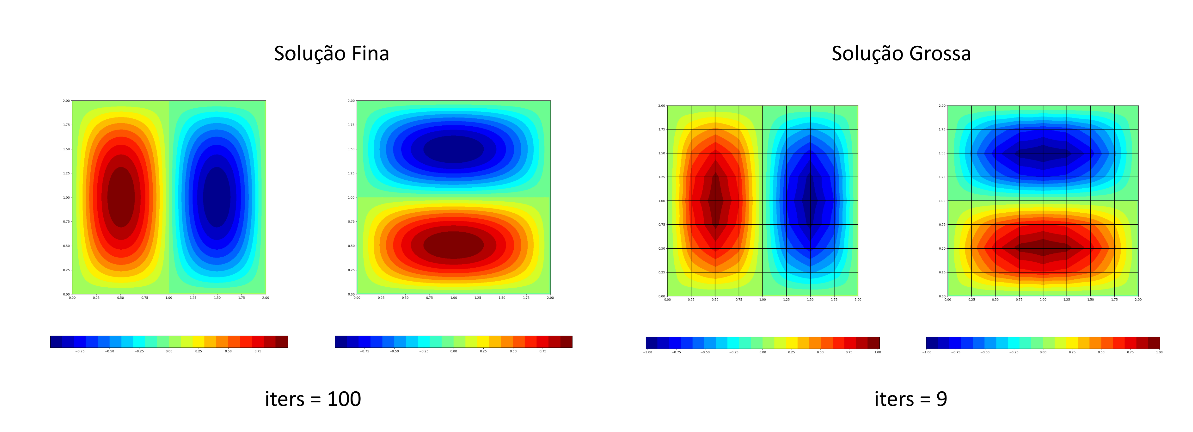
\includegraphics[width=6cm]{chap08/figs/DirichletHomogeneoTemp.png}
\caption{Comparação entre solução do grid fino e do grid grosso. }
\end{figure}


O segundo executado é utilizando a mesma solução anterior mas com domínio $\Omega = [0, 2] \times [0, 1]$, mas agora com condição de Neumann homogênea na fronteira $y=1$. Como a solução não mudou, o lado direito continua da mesma forma que o primeiro caso.

A figura \ref{fig:NeumannHomogeneo} apresenta a solução do grid fino contra a solução do grid grosso.

\begin{figure}[!htbp]
\label{fig:NeumannHomogeneo}
\centering
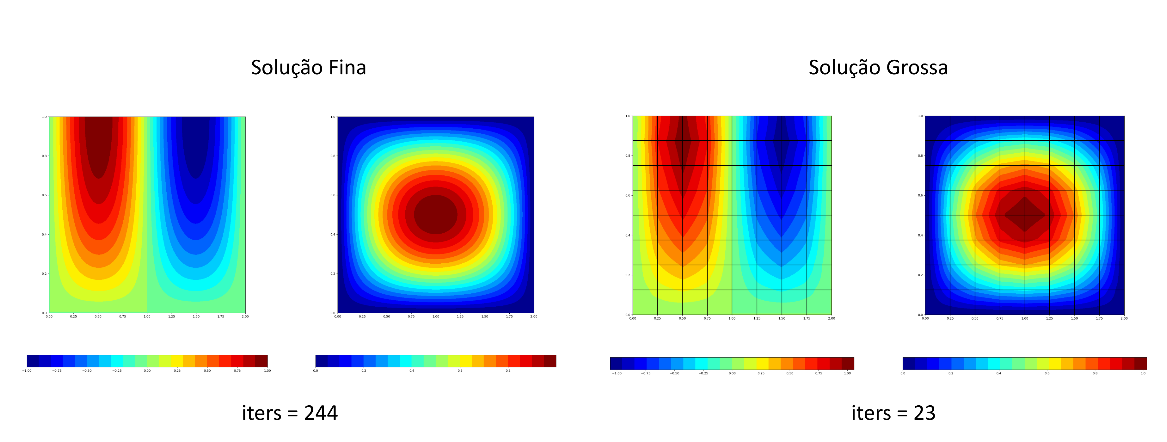
\includegraphics[width=6cm]{chap08/figs/NeumannHomogeneoTemp.png}
\caption{Comparação entre solução do grid fino e do grid grosso. }
\end{figure}



\section{Método Multiescala como pré-condicionador}


Nessa seção, são apresentadas comparações entre o pré-condicionador multiescala e o solver multigrid. Para esse comparação foi utilizado o solver multigrid Pyamg descrito em citacao . Visto a dificuldade da configuração dos solver multigrid, pois esses exigem uma grande quantidade de parâmetros como: a quantidade de níveis devem ser utilizados, quantidade de relaxações em cada nível, qual o tipo de relaxação será utilizada, dentre outras variáveis, foi utilizado o script solver\_diagnotics.py disponibilizado pela equipe do Pyamg no repositório ( citar o repositorio ). Esse script testa sessenta diferentes configurações de solver multigrid e selecionar aquele mais eficiente para o problema proposto.

Os resultados para cada uma das matrizes utilizando mostrou que os solver selecionados para todos os casos possuia no máximo 15 níveis multigrid, e como relaxação utilizavam o "Block Gauss Seidel Sweep". Essa variação do Gauss Seidel é aplicada nos dois sentidos, atualizando primeiramente o valor  $x_1$  do vetor e depois uma iteração atualizando primeiro o valor  $x_n$ . Outro escolha comum para todos os casos, foi a utilização do multigrid como pré-condicionador para o gradiente conjugado.

A figura \ref{fig:reservatorio100x100_1} apresenta o tempo de solução do sistema utilizando o método multiescala como precondicionador para o gradiente conjugado. São apresentados o resíduo ao longo das iterações, o tempo de execução do solver, a quantidade de iterações do solver linear e o tempo da iteração.


\begin{figure}[!htbp]
\label{fig:reservatorio100x100_1}
\centering
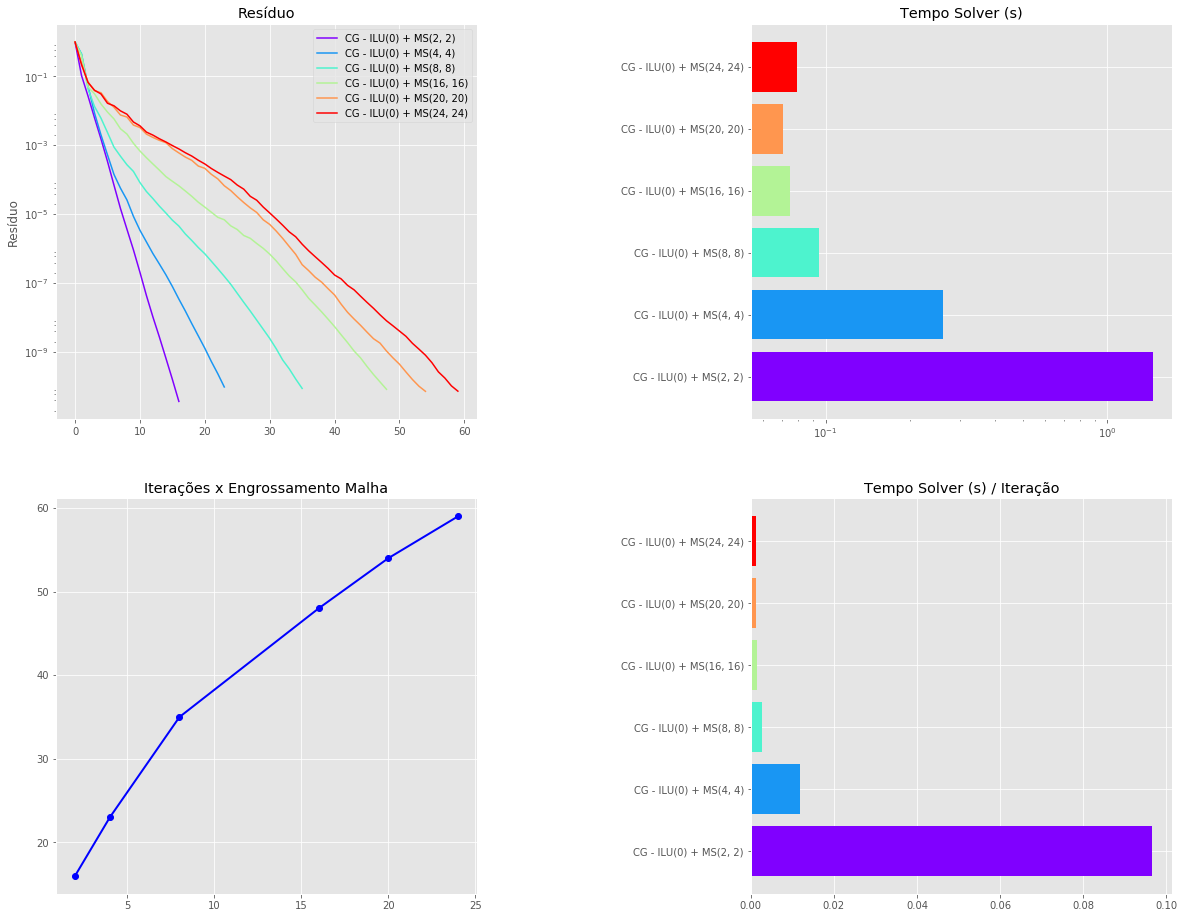
\includegraphics[width=\textwidth]{chap08/figs/reservatorio100x100_1.png}
\caption{Resultados para caso do reservatório 100x100. Histórico do resíduo relativo ao longo das iterações, tempo do solver em segundos, número de iterações em função do fator de engrossamento da malha e tempo do solver por iteração. }
\end{figure}

Um primeiro ponto é o aumento do número de iterações a cada vez que a malha vai ficando mais grossa. Isso ocorre pois a solução do problema vai ficando cada vez mais distante do problema original quanto mais a malha perde resolução. Porém, quanto mais grossa a malha, mais rapidamente o sistema linear do grid grosso é resolvido, pois possui menos variáveis, portanto,  existe uma solução de compromisso entre o engrossamento da malha e a quantidade de iterações que serão necessárias para resolver o sistema linear. No caso do reservatório 100x100, a solução de compromisso fica quando os níveis são engrossados ao se juntar elementos finos 8x8 para criar o novo elemento grosso. 

A figura \ref{fig:reservatorio100x100_2} é apresentado agora a comparação da solução do sistema utilizando o melhor método multiescala com o gradiente conjugado utilizando como precondicionador o ILU(0), ILU(1) e solver multigrid Pyamg. Pode-se notar que apesar da redução de iterações dos método multiescala e do método multigrid, os pré-condicionadores ILU(0) e ILU(1) são mais eficientes na resolução do sistema. 


\begin{figure}[!htbp]
\label{fig:reservatorio100x100_2}
\centering
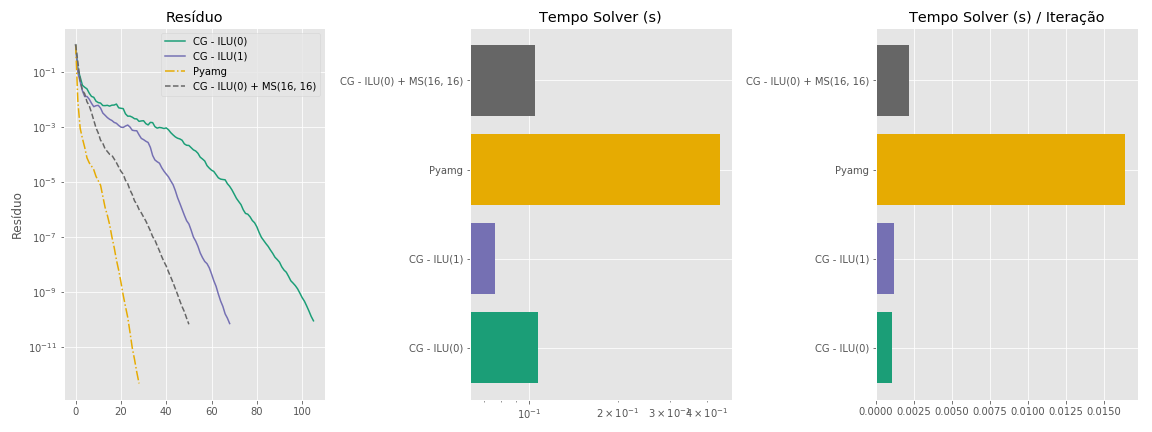
\includegraphics[width=\textwidth]{chap08/figs/reservatorio100x100_2.png}
\caption{Resultados para caso do reservatório 100x100. Histórico do resíduo relativo ao longo das iterações, tempo do solver em segundos, número de iterações em função do fator de engrossamento da malha e tempo do solver por iteração. }
\end{figure}



As figuras \ref{fig:reservatorio320x320_1} e \ref{fig:reservatorio320x320_2} apresentam os mesmos resultados para o caso de 320x320 elementos. Nesse caso, o engrossamento de 20x20 é o que resolve o solver em menor tempo e consegue em um tempo menor que a utilizar apenas ILU(1). 



\begin{figure}[!htbp]
\label{fig:reservatorio320x320_1}
\centering
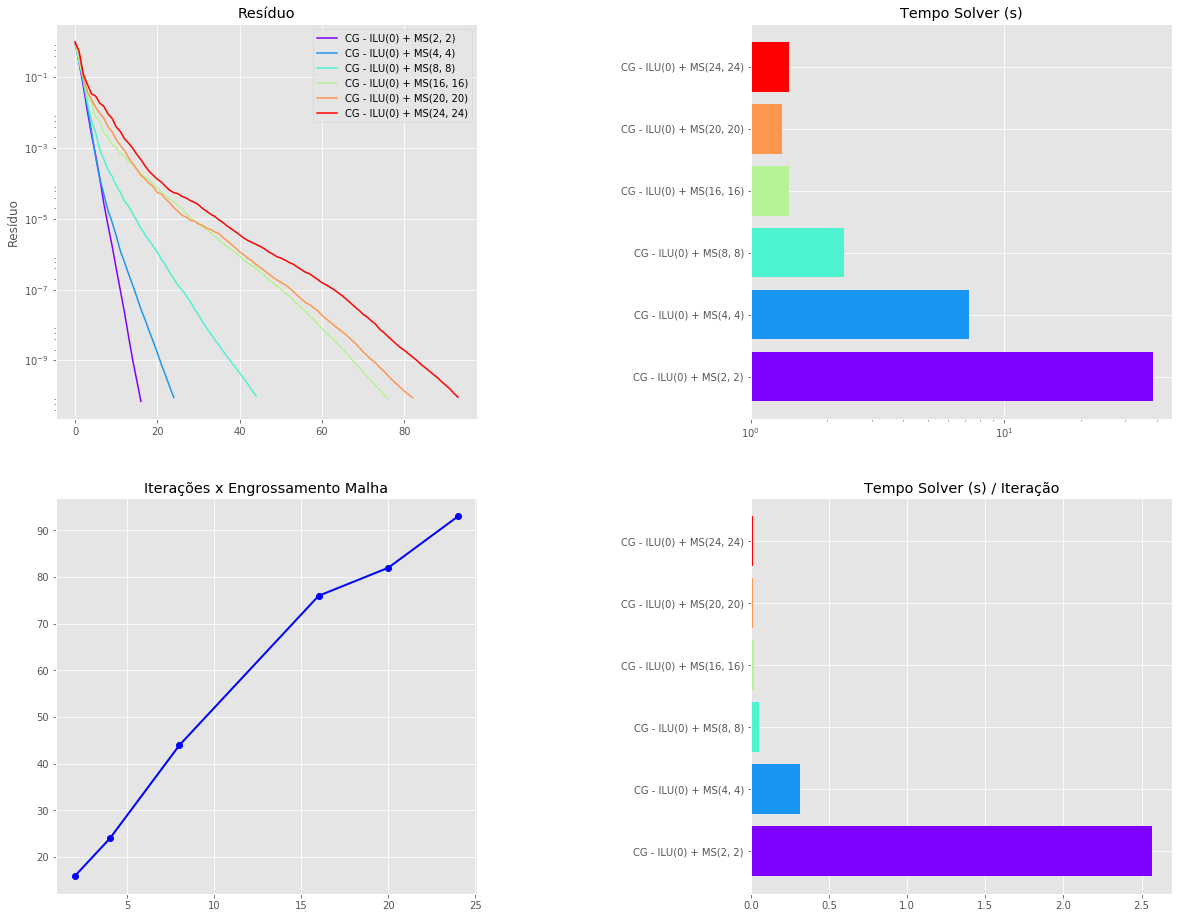
\includegraphics[width=\textwidth]{chap08/figs/reservatorio320x320_1.png}
\caption{Resultados para caso do reservatório 320x320. Histórico do resíduo relativo ao longo das iterações, tempo do solver em segundos, número de iterações em função do fator de engrossamento da malha e tempo do solver por iteração. }
\end{figure}


\begin{figure}[!htbp]
\label{fig:reservatorio320x320_2}
\centering
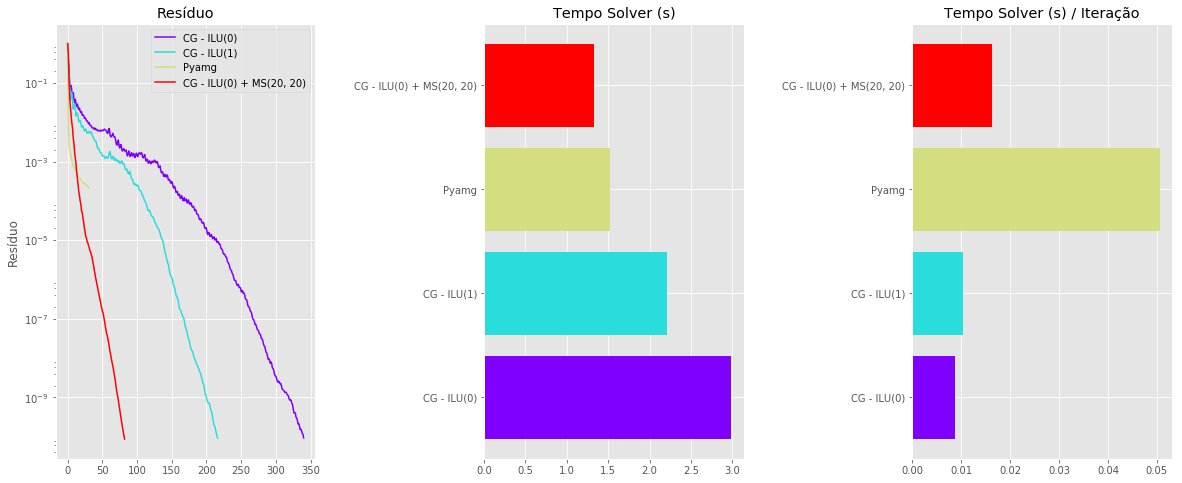
\includegraphics[width=\textwidth]{chap08/figs/reservatorio320x320_2.png}
\caption{Resultados para caso do reservatório 320x320. Histórico do resíduo relativo ao longo das iterações, tempo do solver em segundos, número de iterações em função do fator de engrossamento da malha e tempo do solver por iteração. }
\end{figure}


